\section{Umsetzung}\label{sec:umsetzung}

    \subsection{Resultate}

        Das Praxisrufsystem wurde wie im Kapitel 5 - Konzept beschrieben umgesetzt.
Es wurden die drei Komponenten Mobile Client, Cloud Service und Admin UI implementiert.
Über den angebundenen Messaging Service Firebase Messaging ist es möglich, Benachrichtigungen zwischen Mobile Clients zu versenden.
Cloud Service und Admin UI ermöglichen es dabei die Benachrichtigungen die Versendet werden können und welcher Client welche Benachrichtungen erhalten soll zu konfigurieren.
Weiter wurde mit Amazon Web Services (AWS) eine CI/CD Umgebung aufgebaut, die es erlaubt Cloud Service und das Admin UI zu betreiben und testen.
Diese Umgebung wird dem Kunden als Template dienen, wie er das Praxisrufsystem in der Praxis betreiben kann\footnote{Siehe Anhang Betriebshandbuch}.

Im Rahmen des Projektes wurden damit die Milestones M01 bis M06\footnote{Siehe Kapitel 2.2} erreicht.
Umgesetzt wurden die Milestones mit den folgenden User Stories inklusive aller dazu definierten Features und Szenarien\footnote{Siehe Kapitel 3}:

\begin{itemize}
    \item U01 - Benachrichtigung versenden
    \item U02 - Benachrichtigungen empfangen
    \item U03 - Nur relevante Benachrichtigungen empfangen
    \item U04 - Auf Benachrichtigungen aufmerksam machen
    \item U05 - Verpasste Benachrichtigungen anzeigen
    \item U06 - Fehler beim Versenden von Benachrichtigungen anzeigen
    \item U07 - Konfiguration auf Mobile Client auswählen
    \item U12 - Mehrere Mobile Clients konfigurieren
    \item U13 - Individuelle Konfiguration pro Mobile Client
    \item U14 - Zentrale Konfigurationsverwaltung
    \item T01 - Mobile Client unterstützt IPads
    \item T02 - Mobile Client unterstützt Android Tablets
    \item T03 - Geteilte Code Basis für Android and IOS
    \item T04 - Betrieb mit AWS
\end{itemize}

Die Milestones M06 bis M10 konnten im Rahmen dieses Projektes nicht umgesetzt werden.
Damit sind folgende User Stories ausserhalb des Projektrahmens gefallen:

\begin{itemize}
    \item U08 - Physicher Knopf am Behandlungsstuhl
    \item U09 - Text To Speech für Benachrichtigungen
    \item U10 - Direkte Unterhaltungen zwischen Mobile Clients
    \item U11 - Gruppenunterhaltungen zwischen Mobile Clients
    \item U15 - Konfiguration von direkten Anrufen
    \item U16 - Konfiguration von Gruppenanrufen
\end{itemize}

        \subsubsection{Mobile Client}\label{subsec:mobile-client-realisation}

Dieses Kapitel zeigt die umgesetzten Ansichten des Mobile Clients.
Weitere Informationen zur Bedienung des Mobile Clients sind dem Benutzerhandbuch zu entnehmen\footnote{Siehe Anhang C}.

\subsubsection*{Anmeldung und Konfiguration}

Wird die Mobile Client Applikation zu ersten Mal geöffnet, muss die korrekte Konfiguration geladen werden.
So können Buttons für die benötigten Benachrichtigungen angezeigt und relevante Benachrichtigungen empfangen werden.
In einem ersten Schritt wird dem Benutzer deshalb eine einfache Login-Maske angezeigt.
Darin kann sich der Benutzer mit Benutzername und Passwort anmelden.
War die Anmeldung erfolgreich, werden alle Konfigurationen geladen, die dem Benutzer zur Verfügung stehen.
Die verfügbaren Konfigurationen werden dem Benutzer in einer Liste angezeigt und er wird aufgefordert, die gewünschte Konfiguration auszuwählen.
Nachdem die Auswahl erfolgt ist, wird der Benutzer zur Startseite weitergeleitet.

\begin{figure}[h]
    \centering
    \begin{minipage}[b]{0.4\textwidth}
        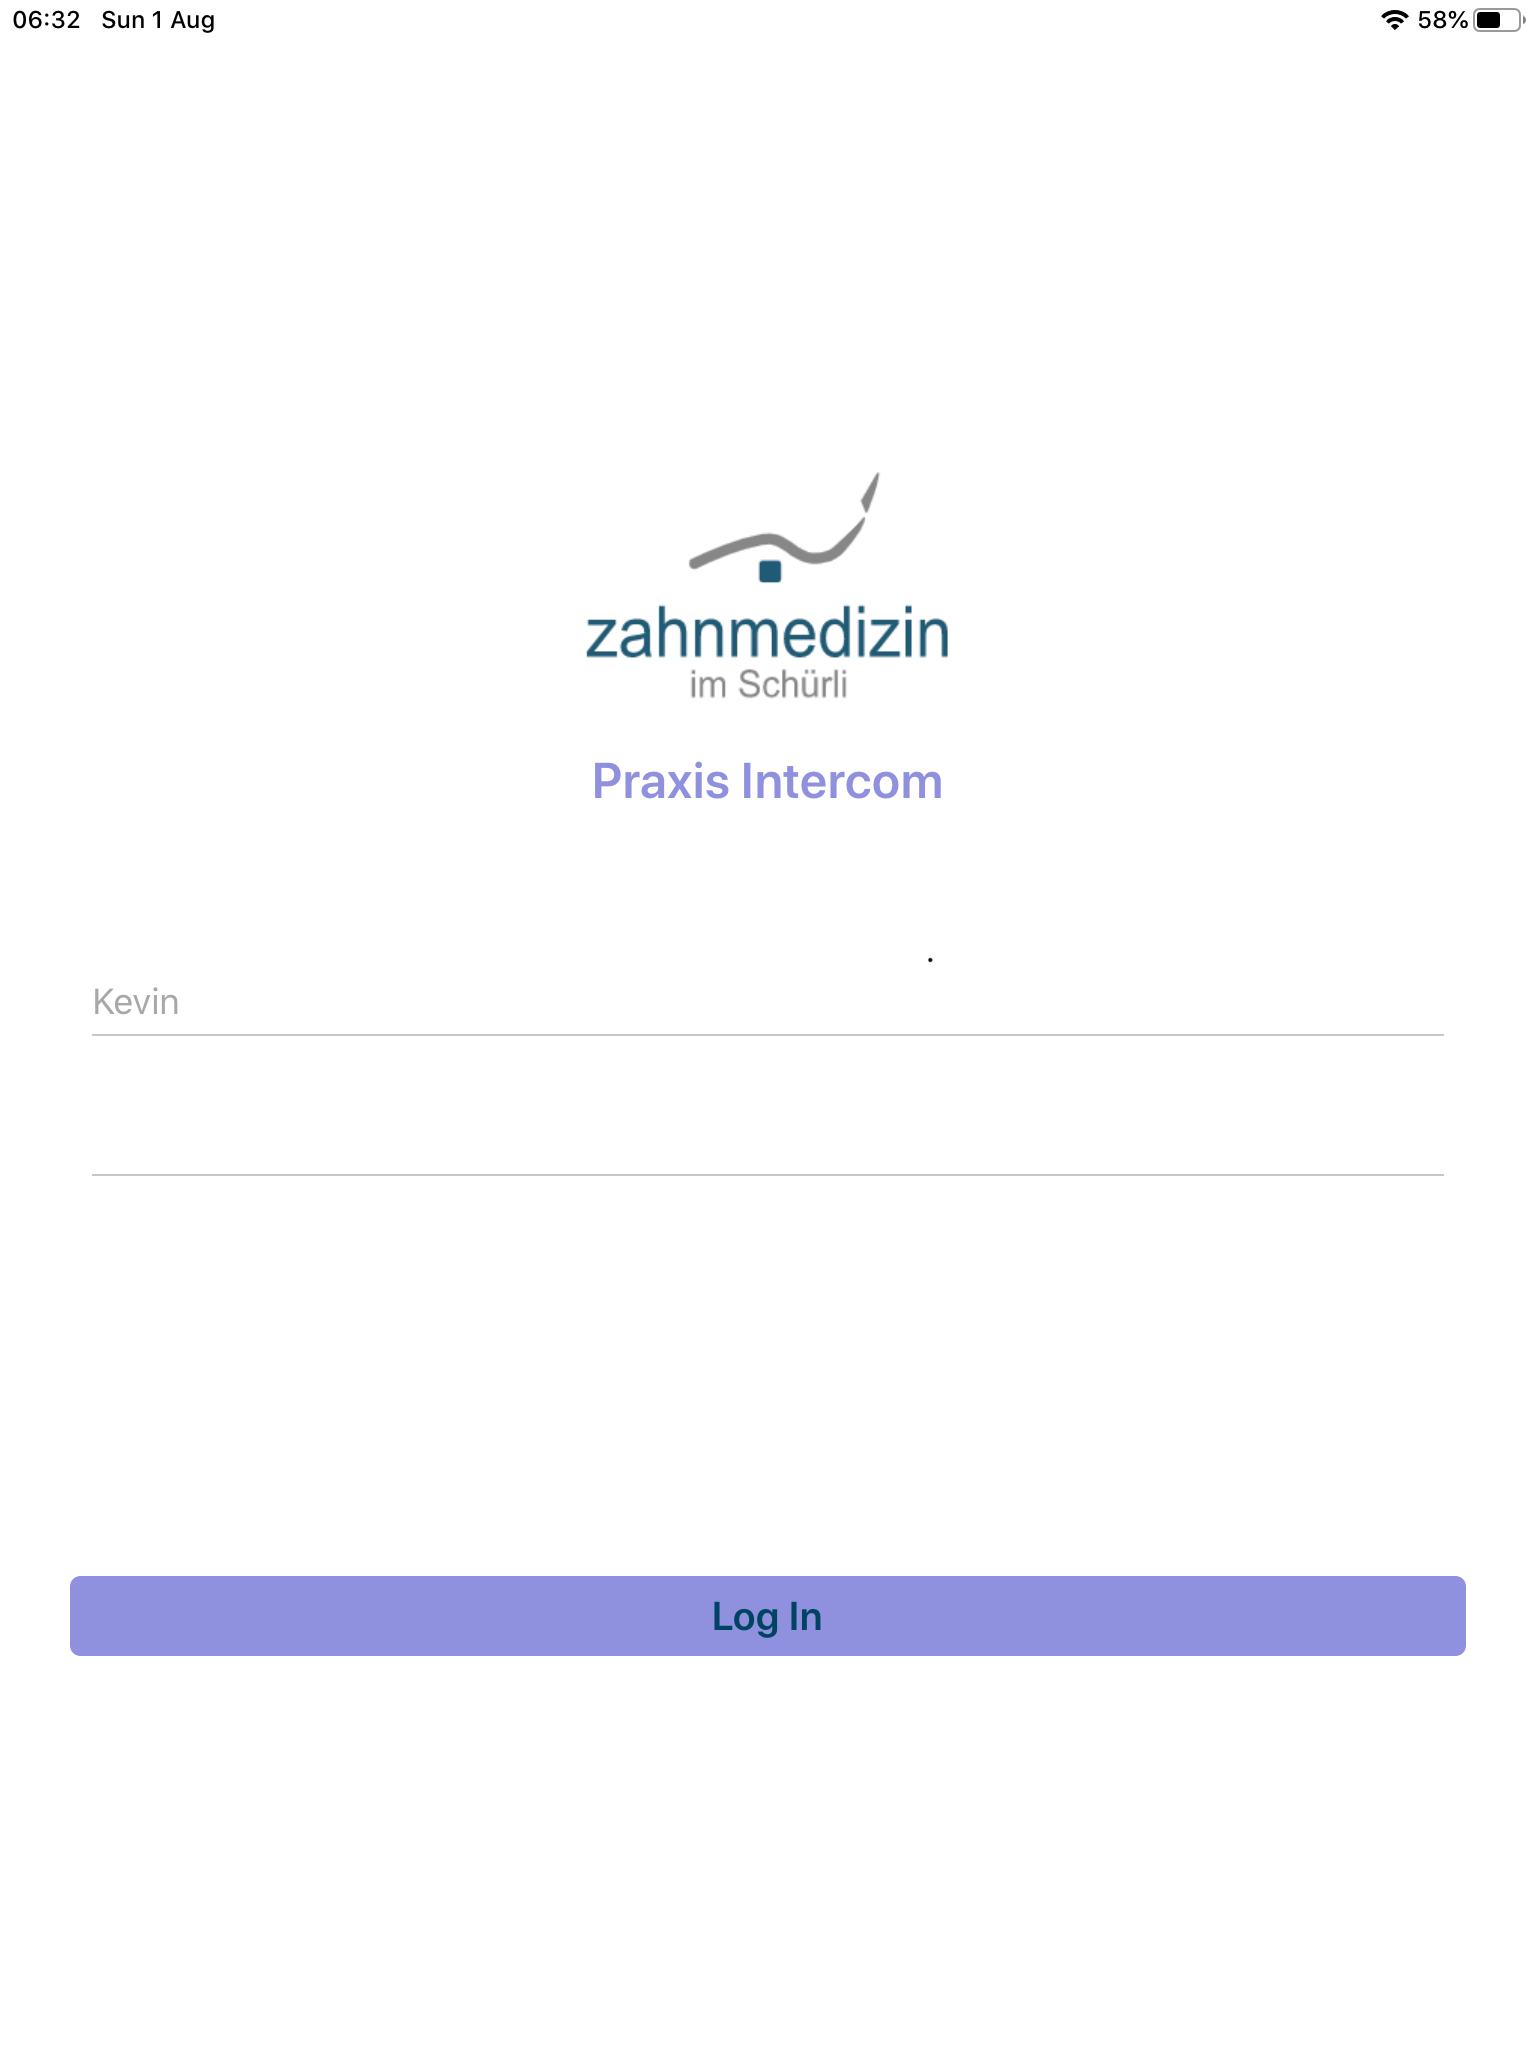
\includegraphics[width=\textwidth]{graphics/screenshots/mobileclient/screenshots-login}
        \caption{Login}
    \end{minipage}
    \hfill
    \begin{minipage}[b]{0.4\textwidth}
        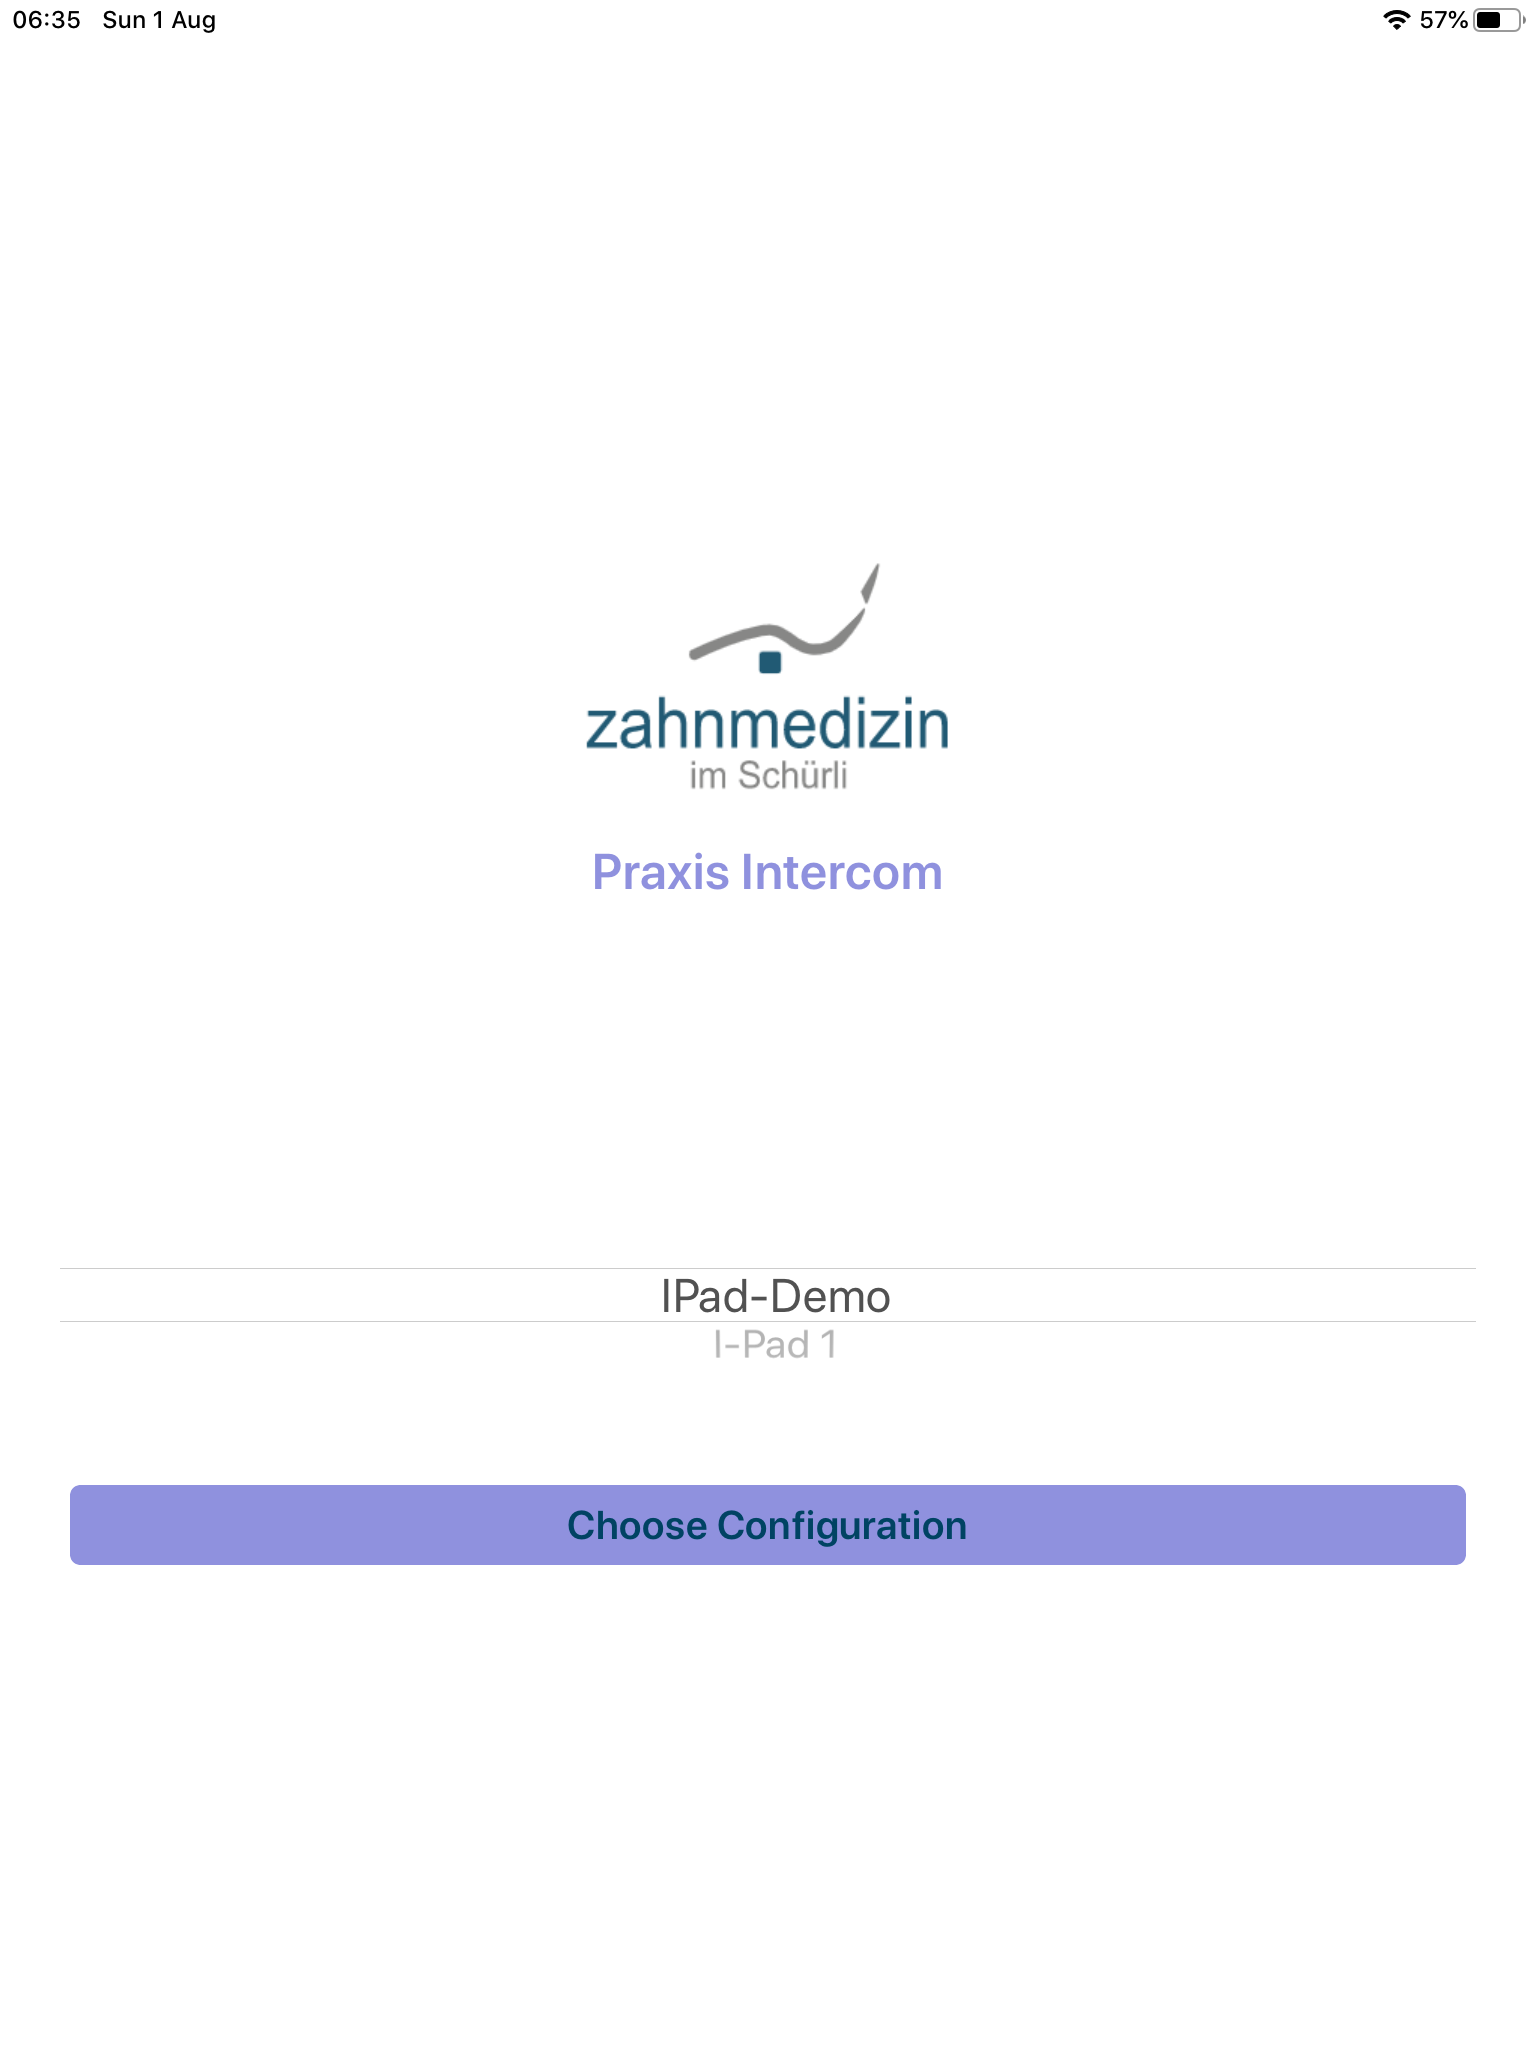
\includegraphics[width=\textwidth]{graphics/screenshots/mobileclient/screenshot-select-config}
        \caption{Konfiguration}
    \end{minipage}
    \label{fig:MobileClient-Screens1}
\end{figure}

\clearpage

\subsubsection*{Benachrichtigungen versenden}

Im Tab Home der Startseite werden Buttons angezeigt, um Benachrichtigungen zu versenden.
Die Buttons werden dynamisch aus der geladenen Konfiguration generiert.
Dabei gibt die Konfiguration den Text vor, der auf dem Button angezeigt wird.
Der Inhalt der Benachrichtigung, die der Button auslöst, ist in der Konfiguration im Cloud Service hinterlegt.

Tippt der Benutzer auf einen der Buttons, wird die entsprechende Benachrichtigung versendet.
Die Vermittlung, an die relevanten Empfänger übernimmt dabei der Cloud Service.
Dieser entscheidet anhand der vorhandenen Konfiguration, welchen Clients die Benachrichtigung zugestellt wird.
Schlägt das Versenden der Benachrichtigung an mindestens einen Empfänger fehl, wird dies dem Benutzer angezeigt.
Der Benutzer hat dann die Möglichkeit, das Versenden an diese Empfänger wiederholen.

\begin{figure}[h]
    \centering
    \begin{minipage}[b]{0.4\textwidth}
        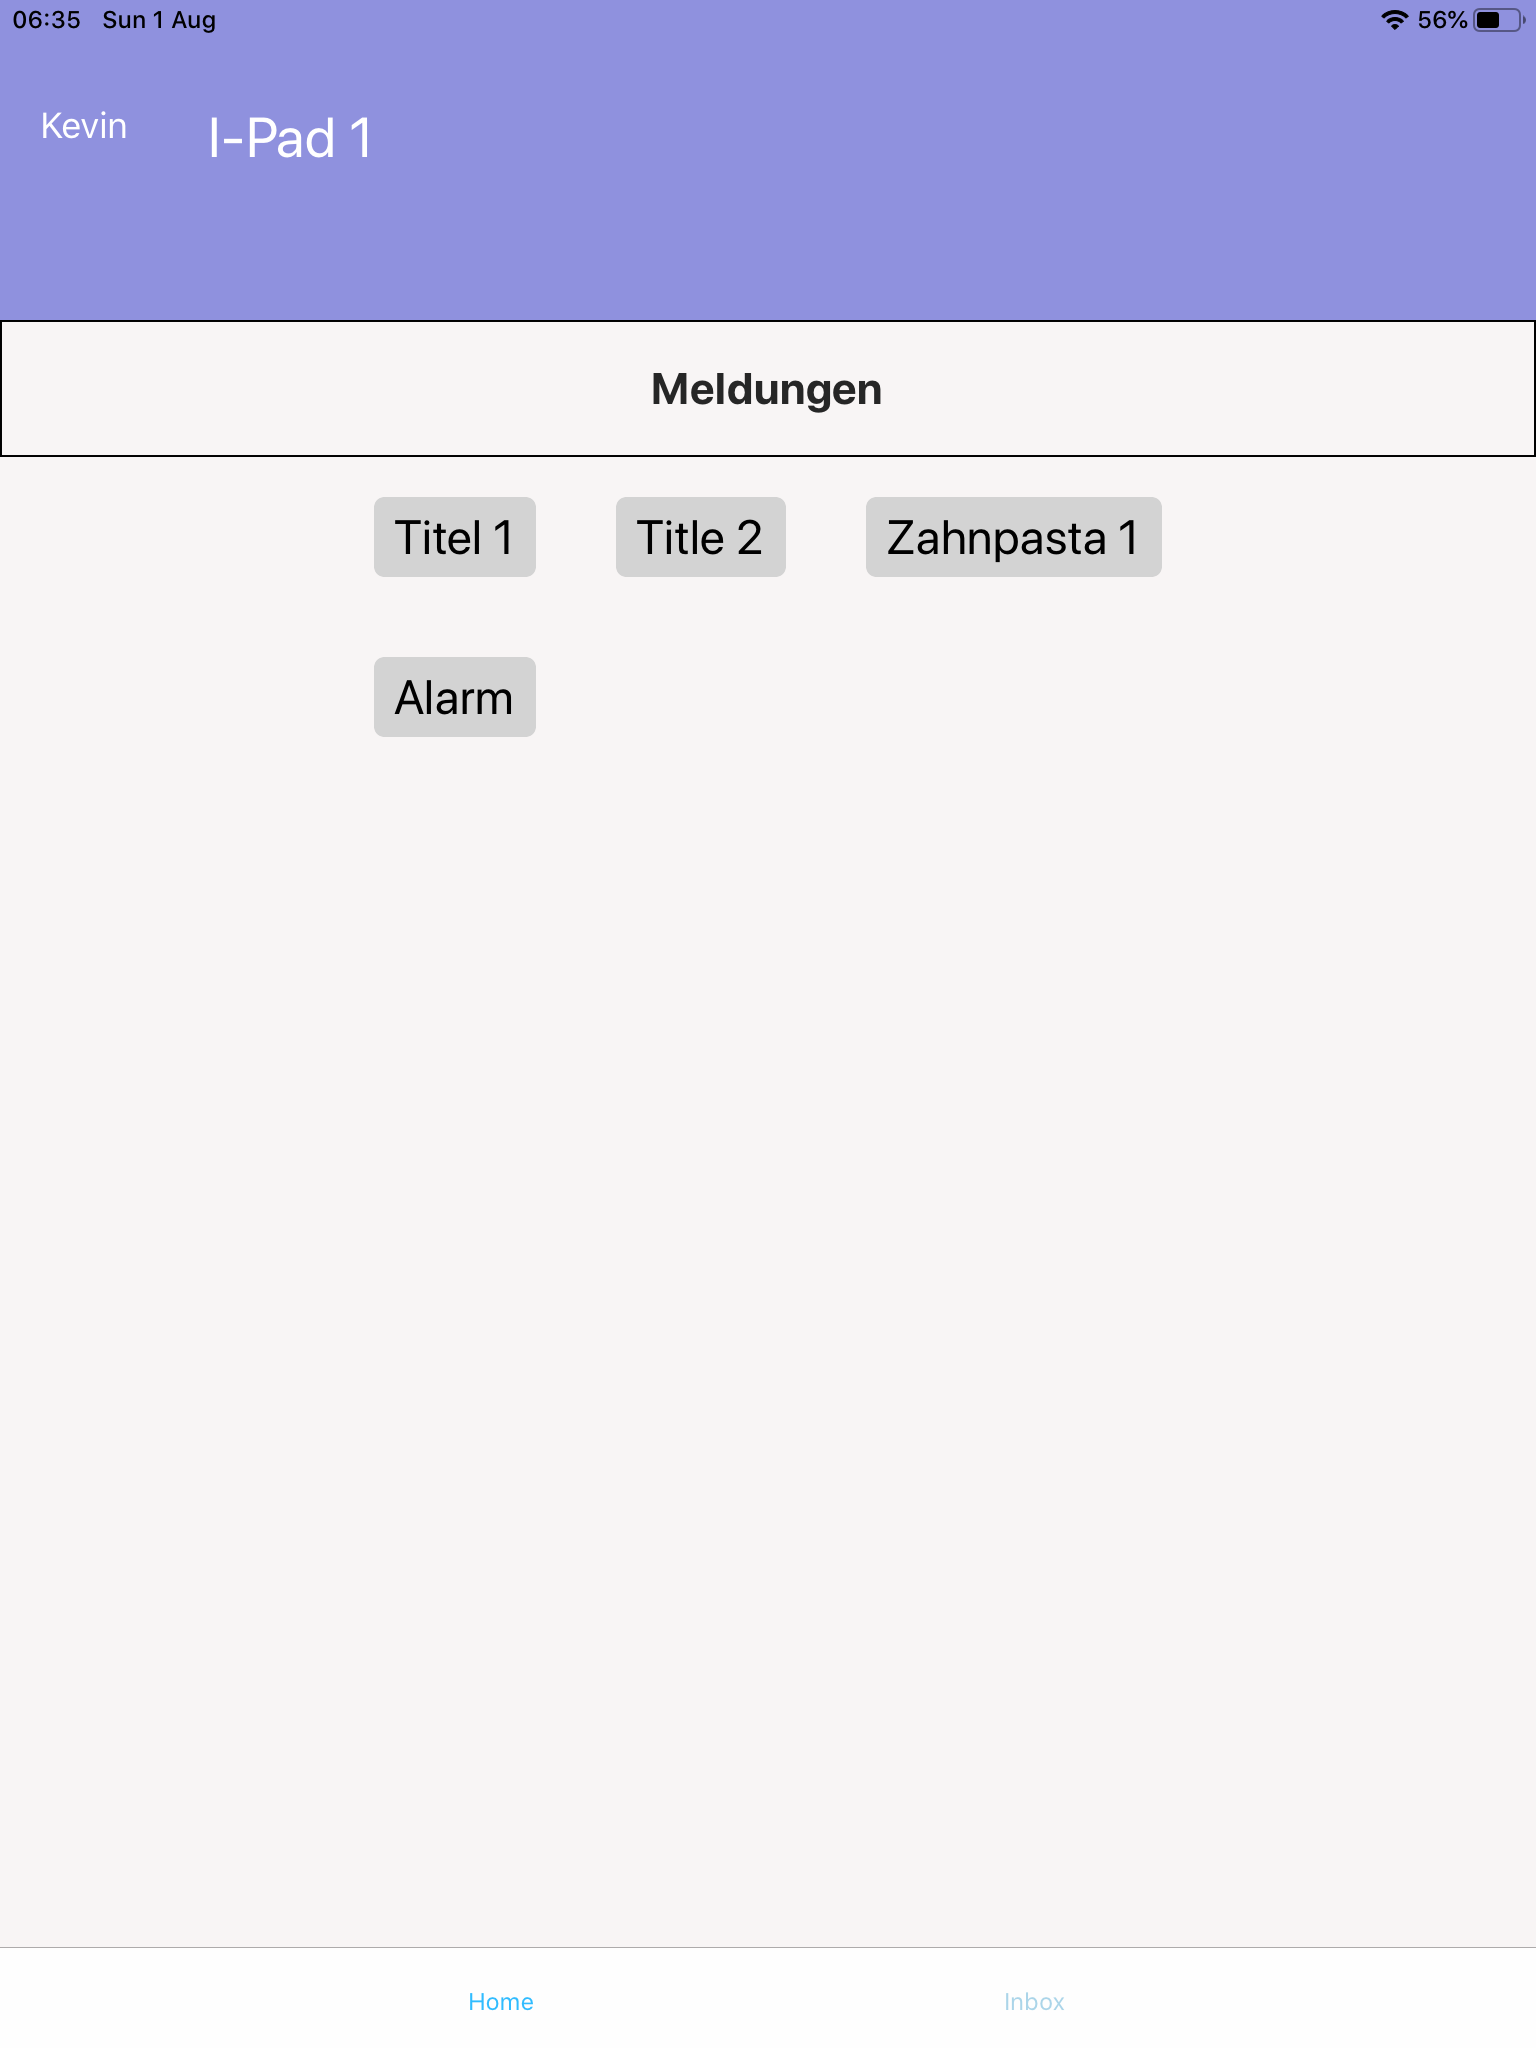
\includegraphics[width=\textwidth]{graphics/screenshots/mobileclient/screenshot-homescreen}
        \caption{Home}
    \end{minipage}
    \hfill
    \begin{minipage}[b]{0.4\textwidth}
        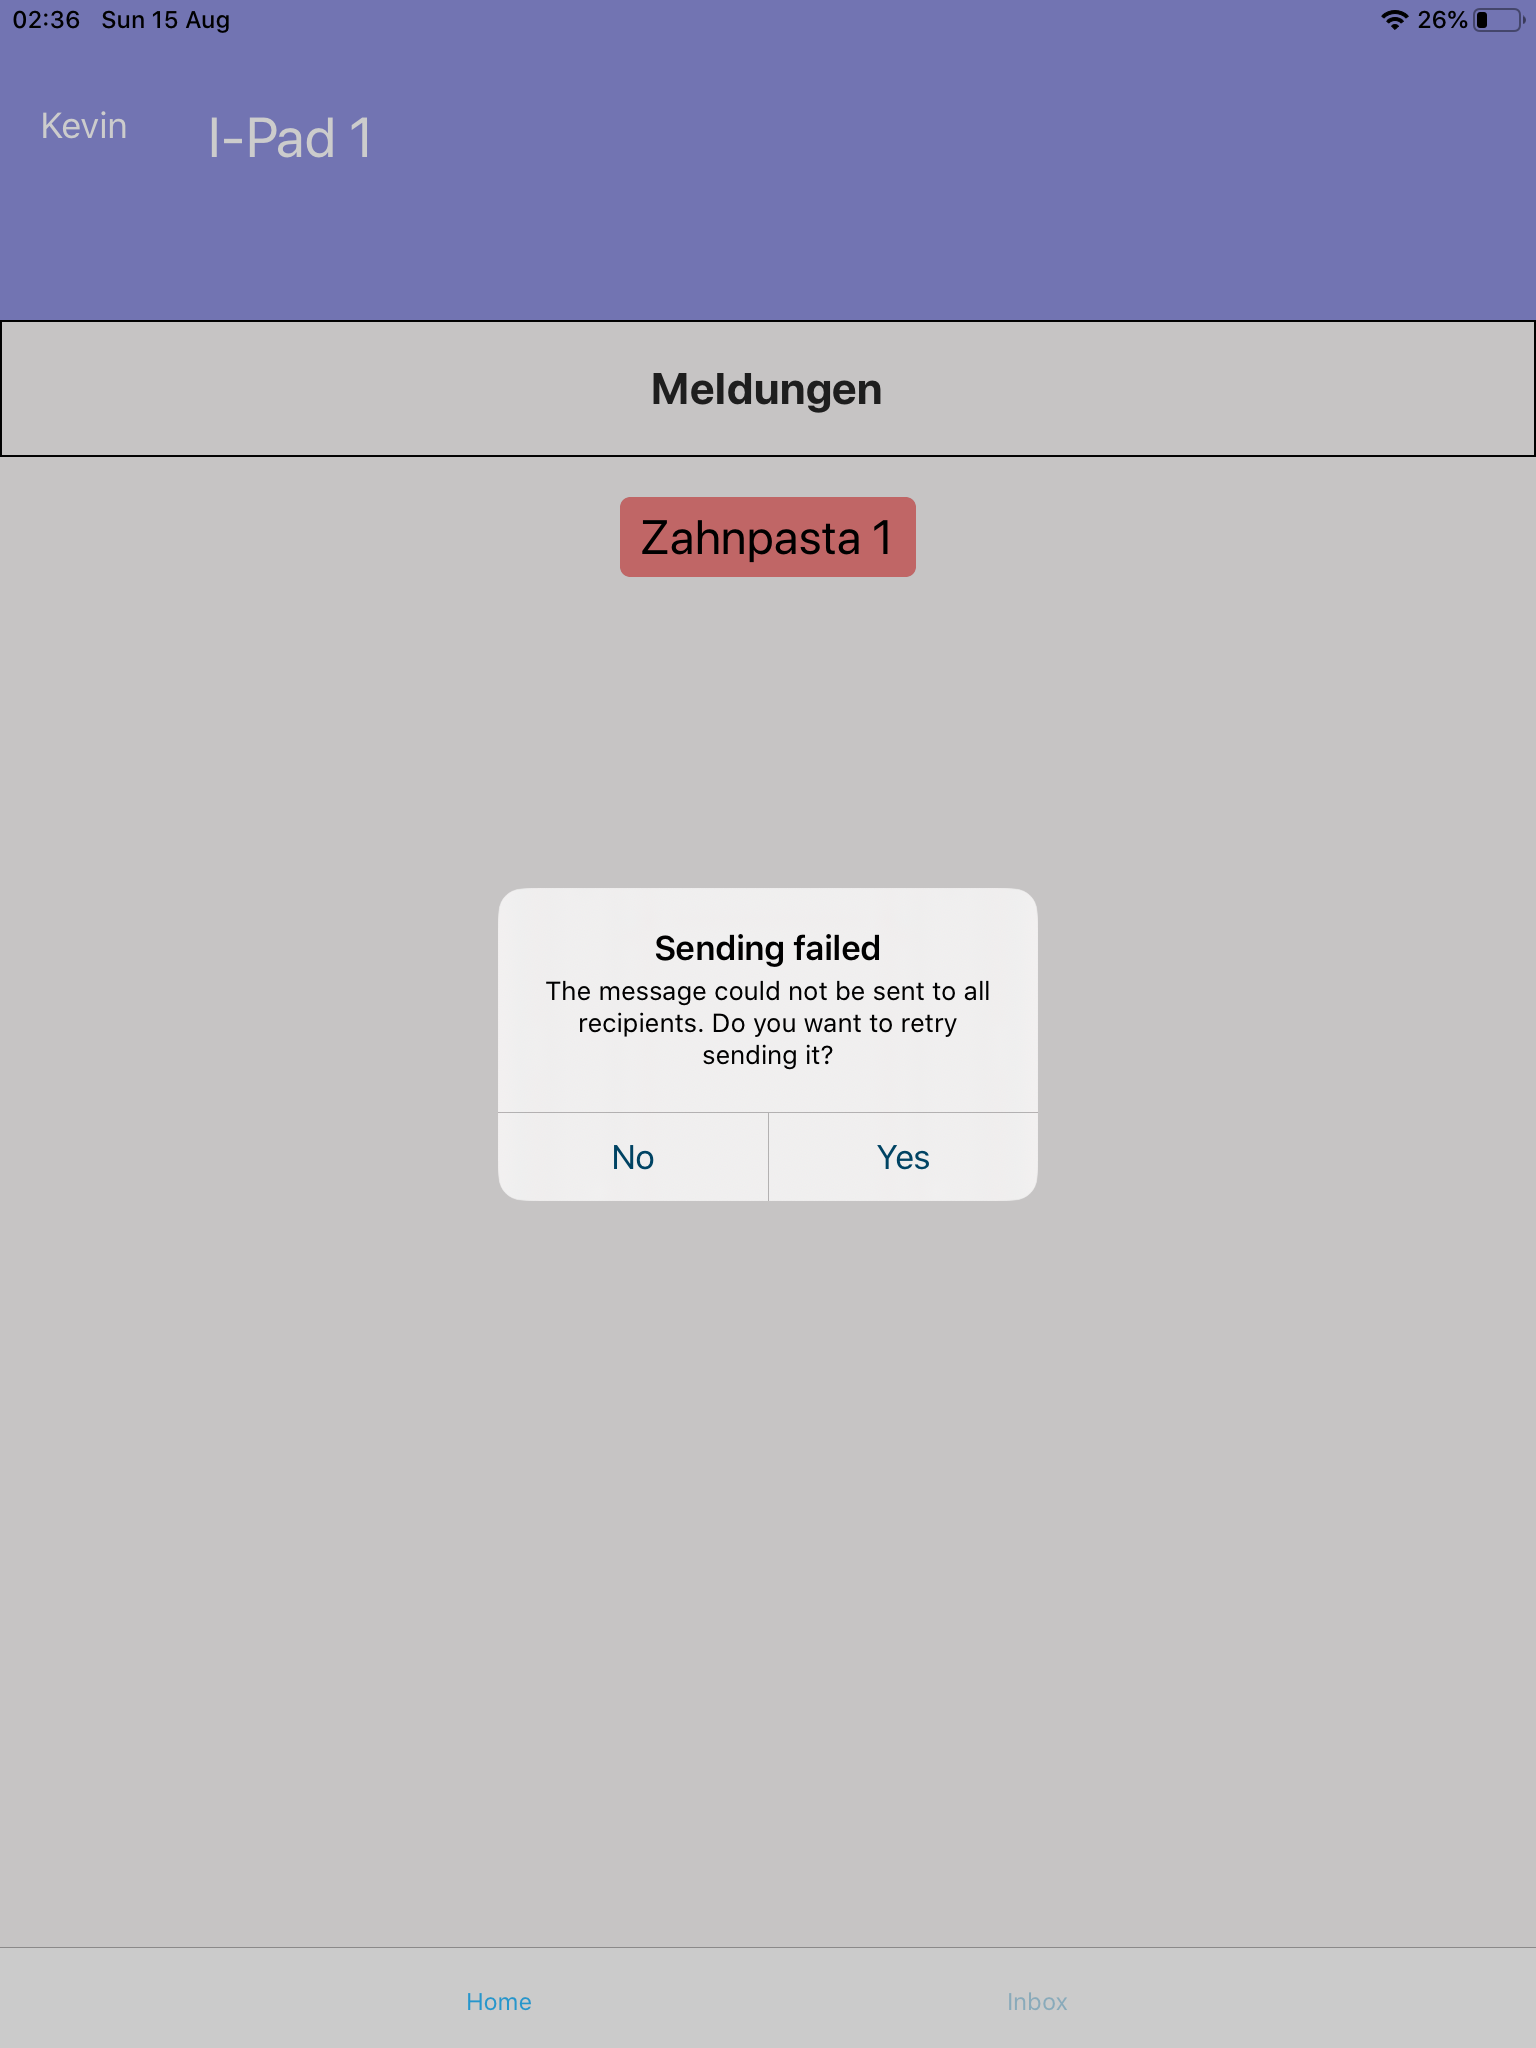
\includegraphics[width=\textwidth]{graphics/screenshots/mobileclient/screenshot-retry}
        \caption{Retry}
    \end{minipage}
    \label{fig:MobileClient-Screens2}
\end{figure}

\clearpage

\subsubsection*{Benachrichtigungen empfangen}

Wurde eine Benachrichtigung empfangen, ertönt ein Audio Signal und die Benachrichtigung ist im Tab Inbox auf der Startseite ersichtlich.
Durch Klick auf einen der Einträge in der Liste, kann der Benutzer die empfangene Benachrichtigung quittieren.
Wenn die Inbox Benachrichtigungen enthält, die nicht quittiert wurden, wiederholt der Client im Abstand von 30 Sekunden.
Die Quittierung von Benachrichtigungen erfolgt nur lokal auf dem Gerät.
Der Versender wird nicht über die Quittierung benachrichtigt.
Wurde eine Benachrichtigung im Hintergrund empfangen, wird diese als Push-Benachrichtigung auf dem Gerät angezeigt.
Auch wenn die Benachrichtigung im Hintergrund empfangen wurde, wird diese in der Inbox angezeigt.

\begin{figure}[h]
    \centering
    \begin{minipage}[b]{0.4\textwidth}
        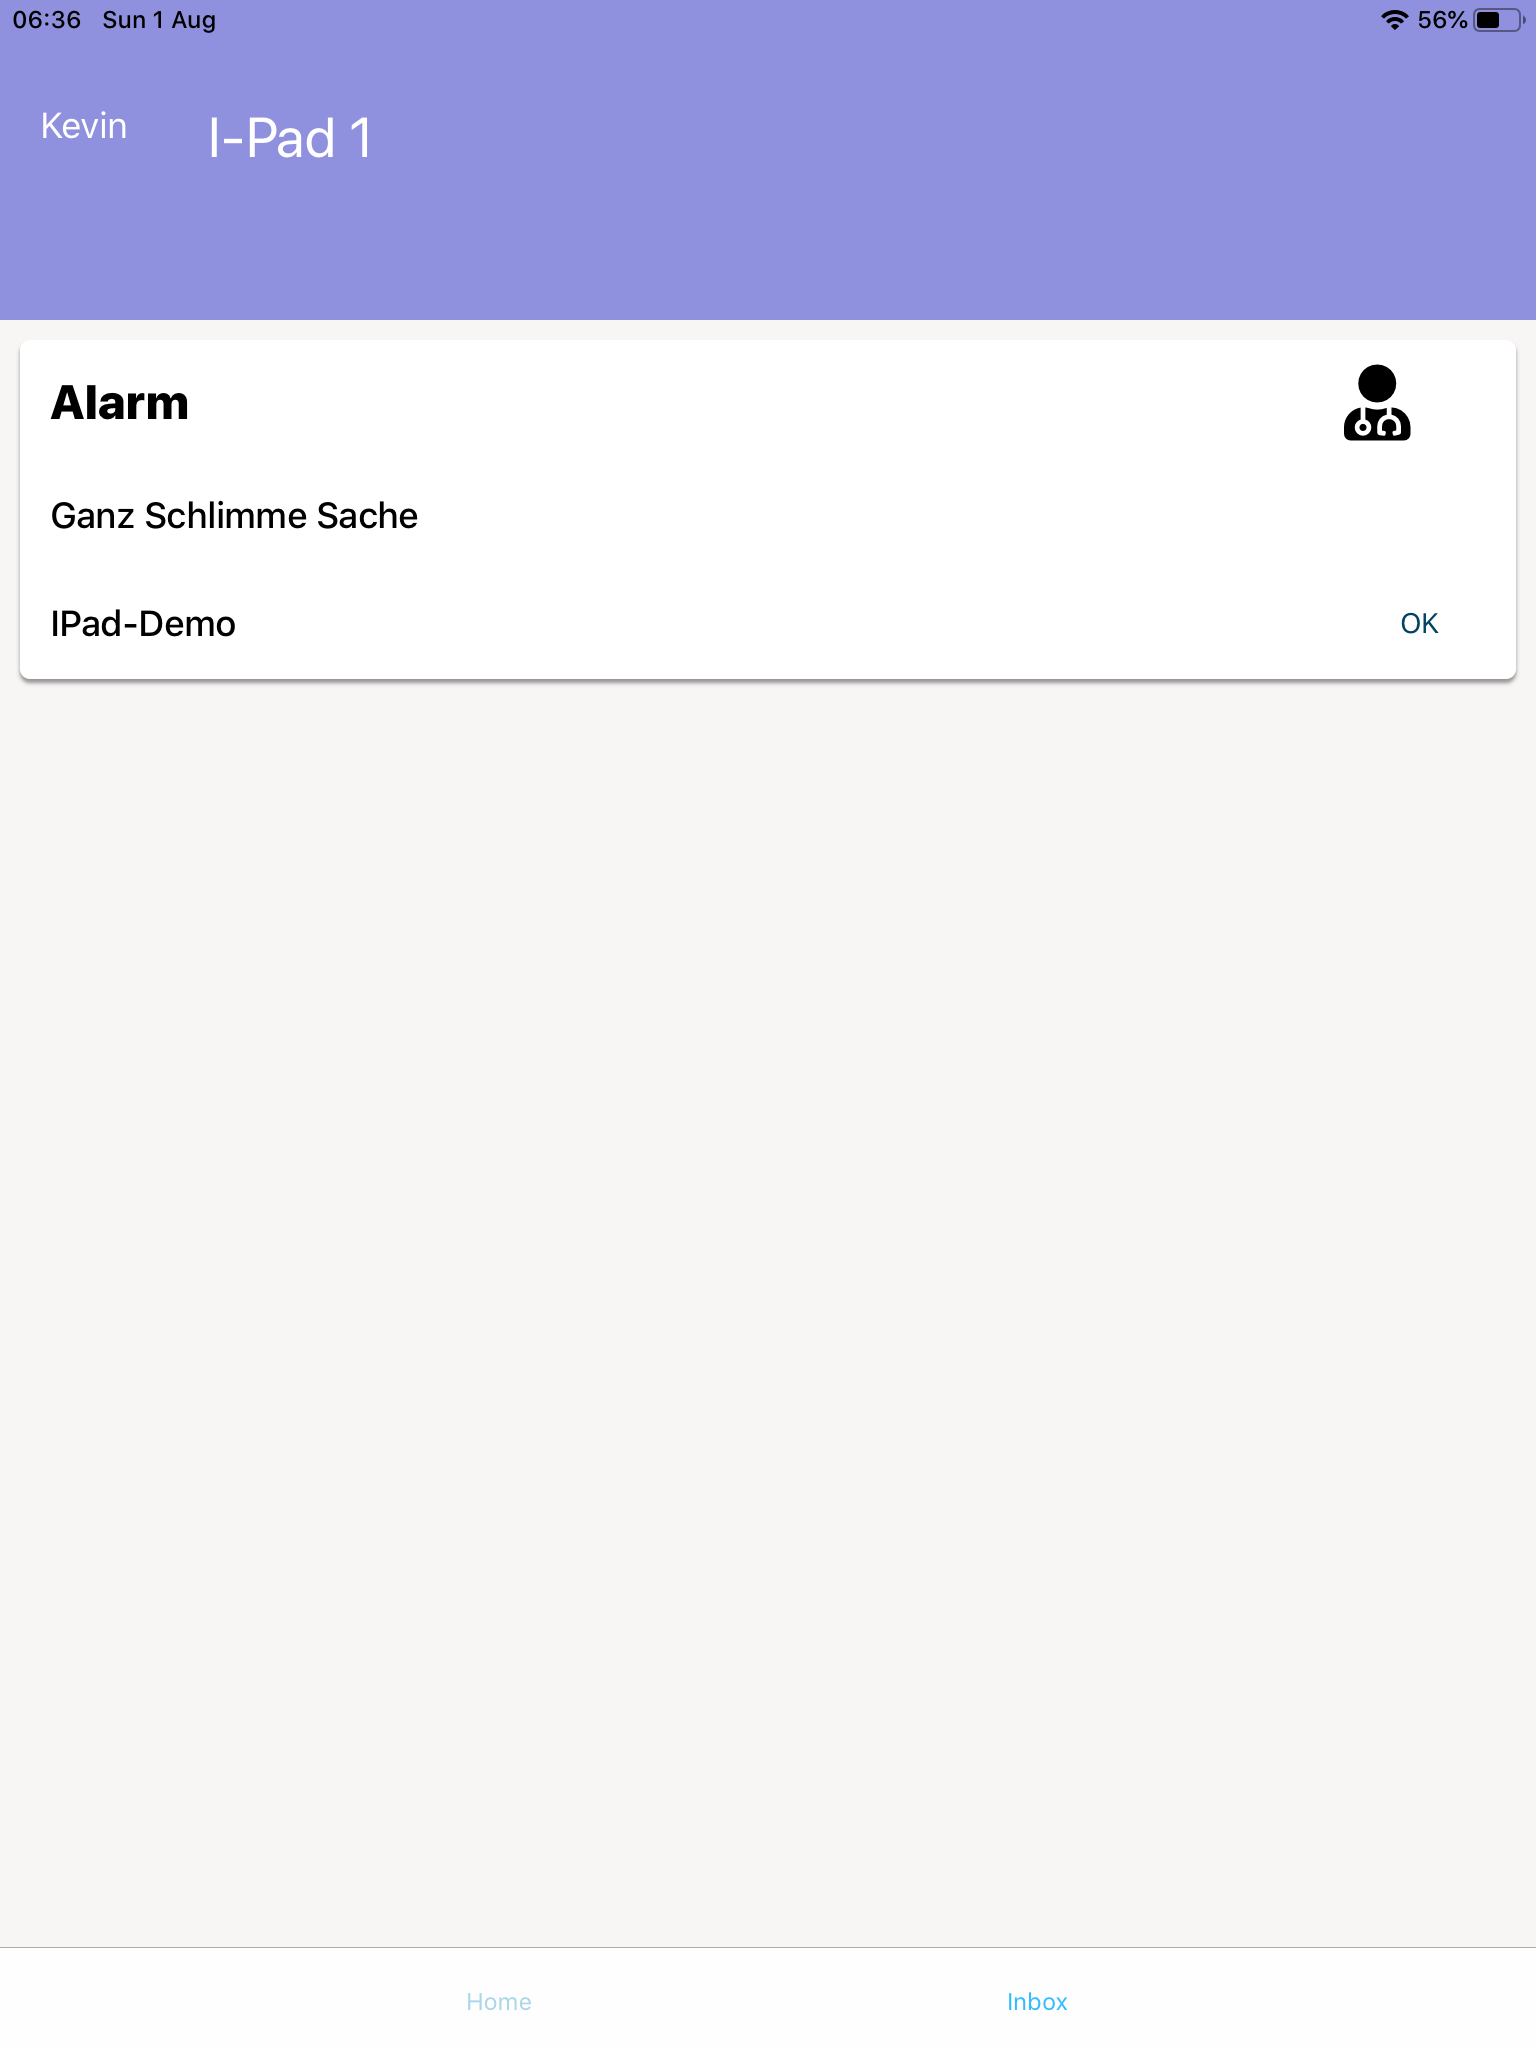
\includegraphics[width=\textwidth]{graphics/screenshots/mobileclient/screenshots-inbox}
        \caption{Inbox}
    \end{minipage}
    \hfill
    \begin{minipage}[b]{0.4\textwidth}
        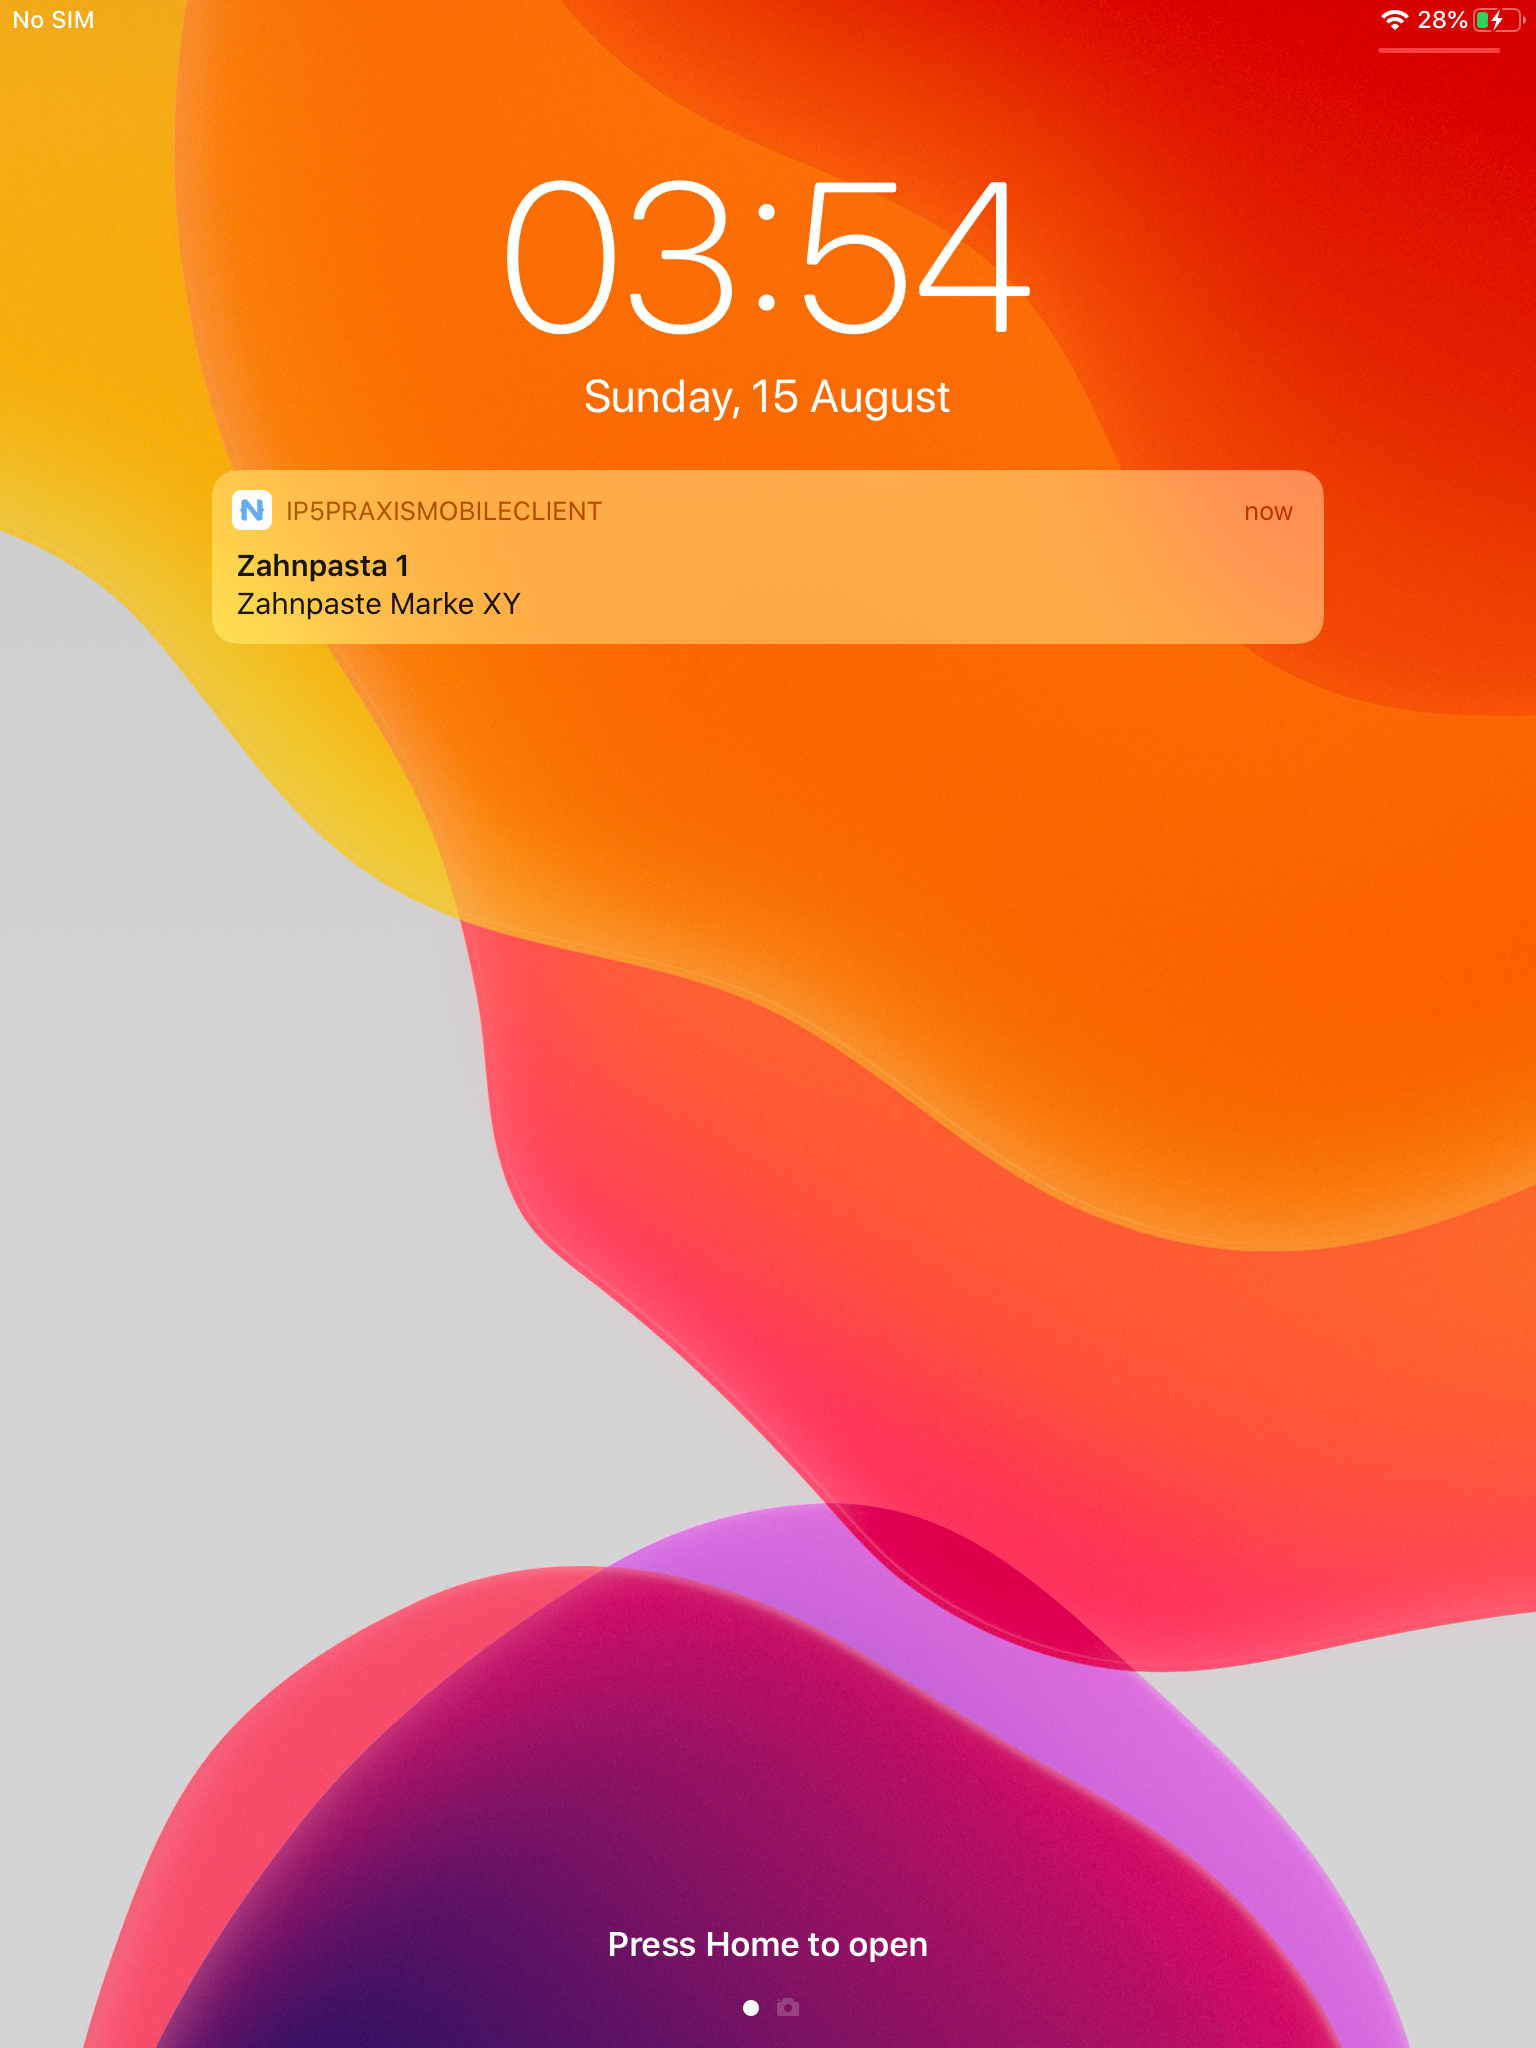
\includegraphics[width=\textwidth]{graphics/screenshots/mobileclient/screenshot-push}
        \caption{Push Benachrichtigung}
    \end{minipage}
    \label{fig:MobileClient-Screens3}
\end{figure}

\clearpage


        
\subsection{Cloud Service}\label{subsec:cloud-service}

\subsubsection{Architektur}

Es gibt deren Domänen 2. Configuration und Notification.

So quasi als ob man 2 Microservices haben kann. Aber wär halt doof das für den stand jetzt schon so zu trennen, deshalb vorerst mal erst ein einzelnes.

\clearpage

\subsubsection{Domänenmodell}


Für die beiden Domänen gibt es natürlich auch so n paar Diagramme. Die gibts jetzt hier:


\subsubsection*{Domäne Configuration}

\begin{figure}[h]
    \centering
    \begin{minipage}[b]{1.0\textwidth}
        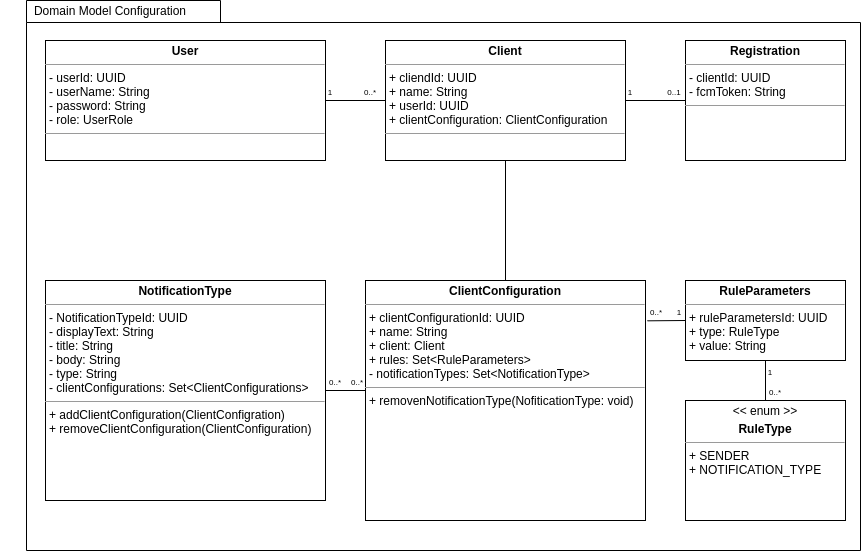
\includegraphics[width=\textwidth]{graphics/Class_Configuration_Domain}
        \caption{Domänenmodell Configuration}
    \end{minipage}
\end{figure}

\clearpage
\subsubsection*{Domäne Notification}

\begin{figure}[h]
    \centering
    \begin{minipage}[b]{1.0\textwidth}
        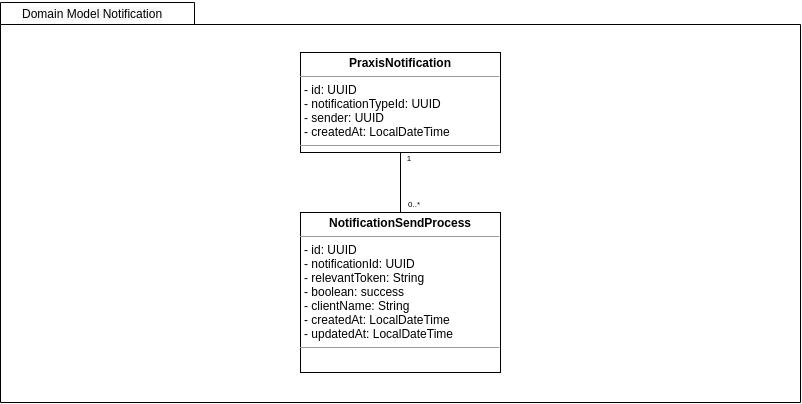
\includegraphics[width=\textwidth]{graphics/Class_Notification_Domain}
        \caption{Domänenmodell Notification}
    \end{minipage}
\end{figure}

\clearpage
\subsubsection*{Rules Engine}

Strategy Pattern mit Spring is noch nice.

\begin{figure}[h]
    \centering
    \begin{minipage}[b]{1.0\textwidth}
        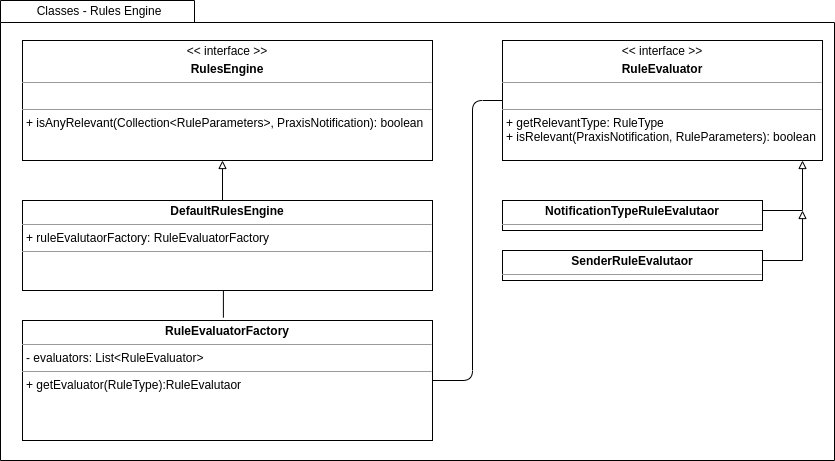
\includegraphics[width=\textwidth]{graphics/Class_Configuration_RulesEngine}
        \caption{Klassendiagramm Rules Engine}
    \end{minipage}
\end{figure}



\clearpage
\subsubsection{API}

S gibt da n paar controller und die brauchen ein paar services.

\clearpage
\subsubsection{Laufzeitmodell}

\clearpage


\subsubsection{Admin UI}

\begin{figure}[h]
    \centering
    \begin{minipage}[b]{0.4\textwidth}
        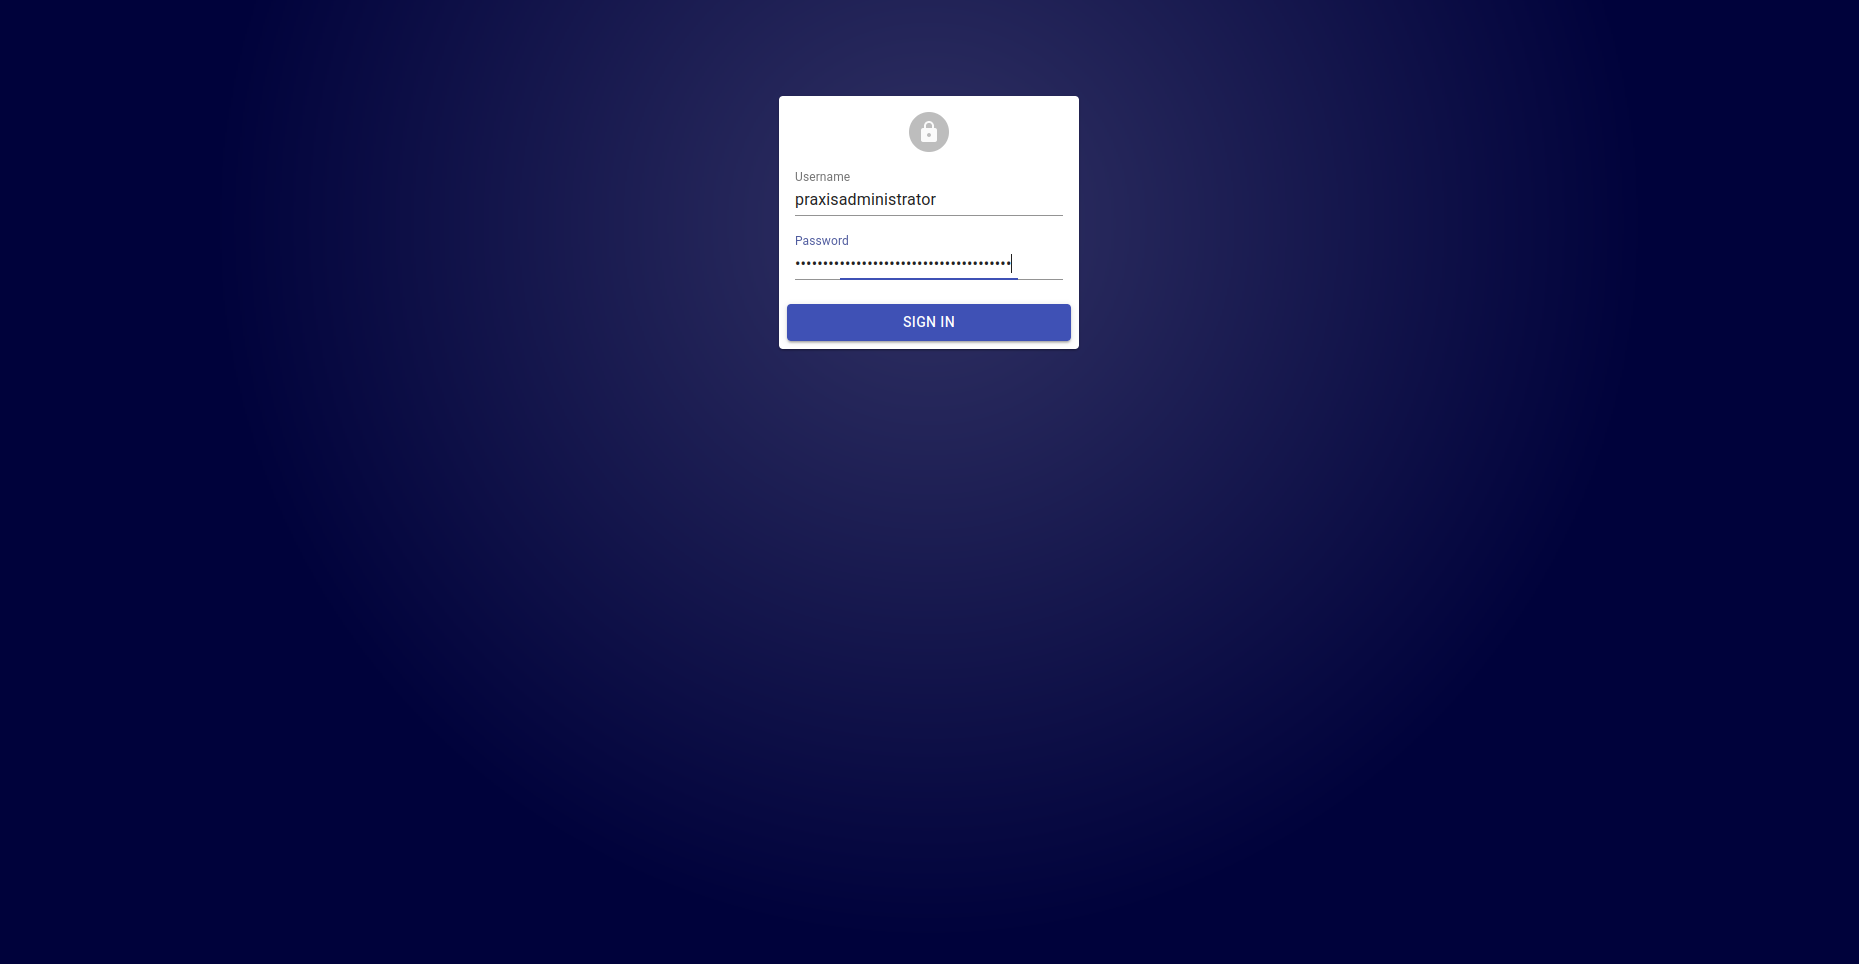
\includegraphics[width=\textwidth]{graphics/screenshots/adminui/login}
        \caption{Login}
    \end{minipage}
    \hfill
    \begin{minipage}[b]{0.4\textwidth}
        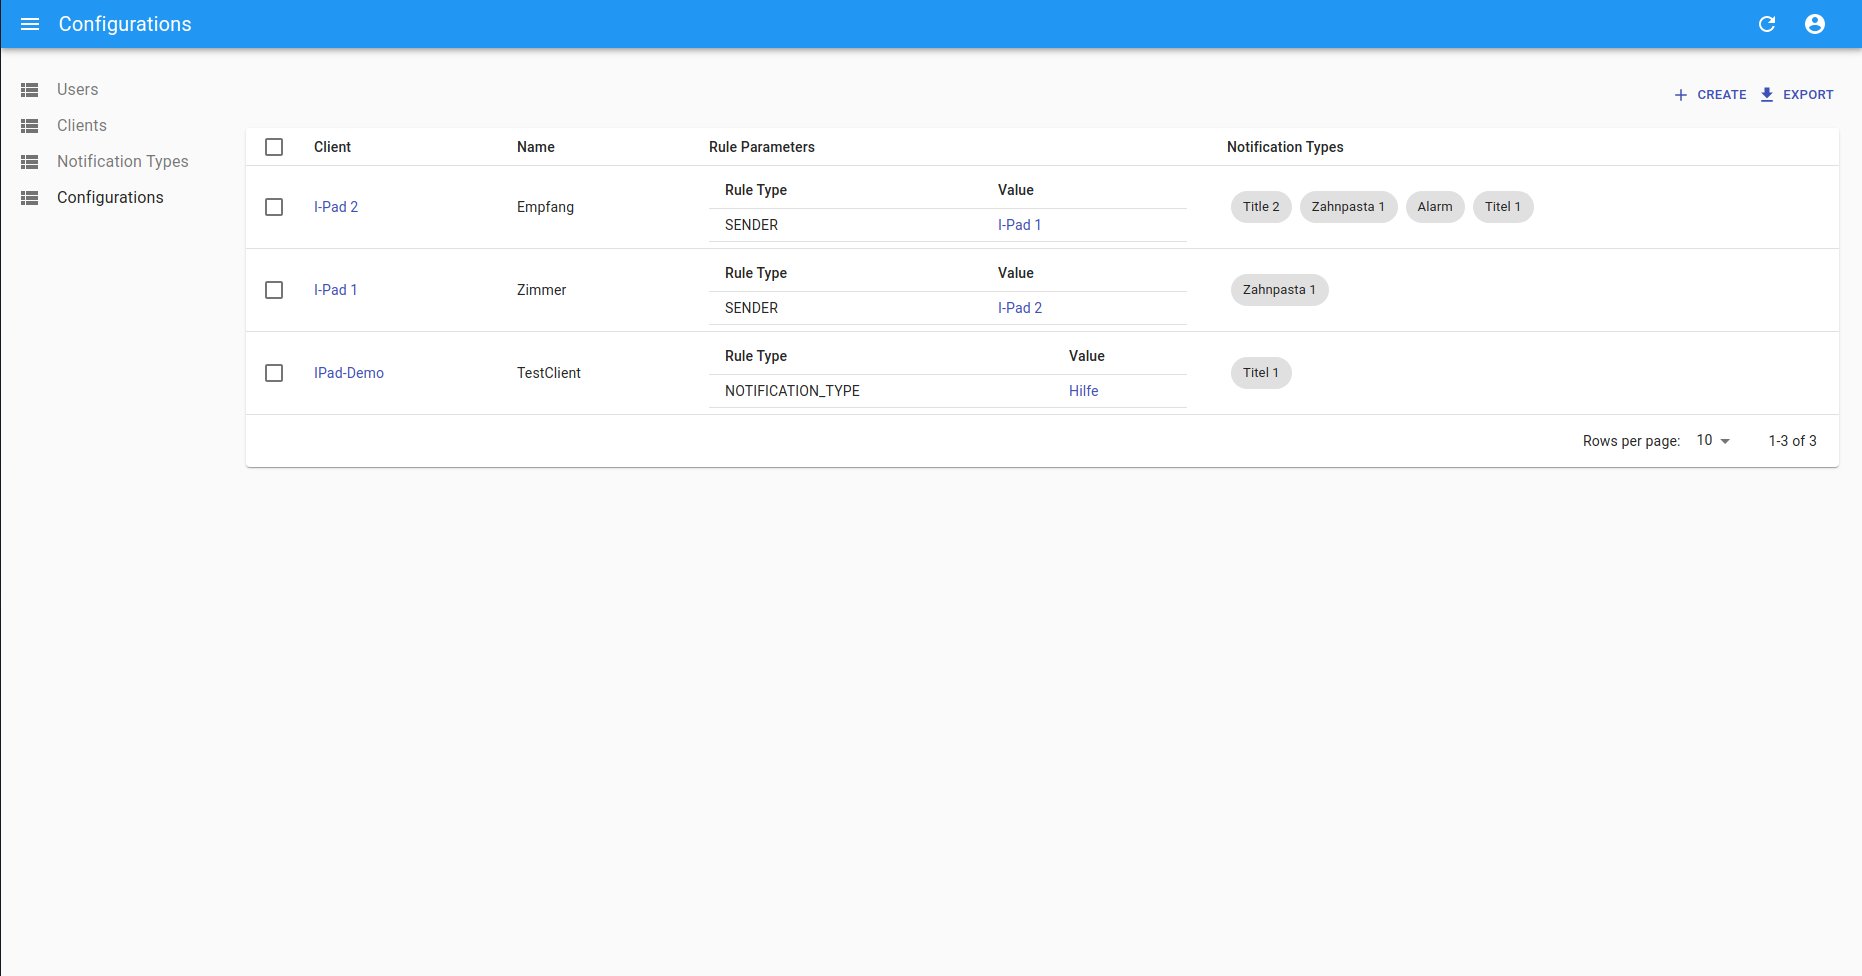
\includegraphics[width=\textwidth]{graphics/screenshots/adminui/configuration-all}
        \caption{Configuration Overview}
    \end{minipage}
    \label{fig:AdminUI-Screens1}
\end{figure}

\begin{figure}[h]
    \centering
    \begin{minipage}[b]{0.4\textwidth}
        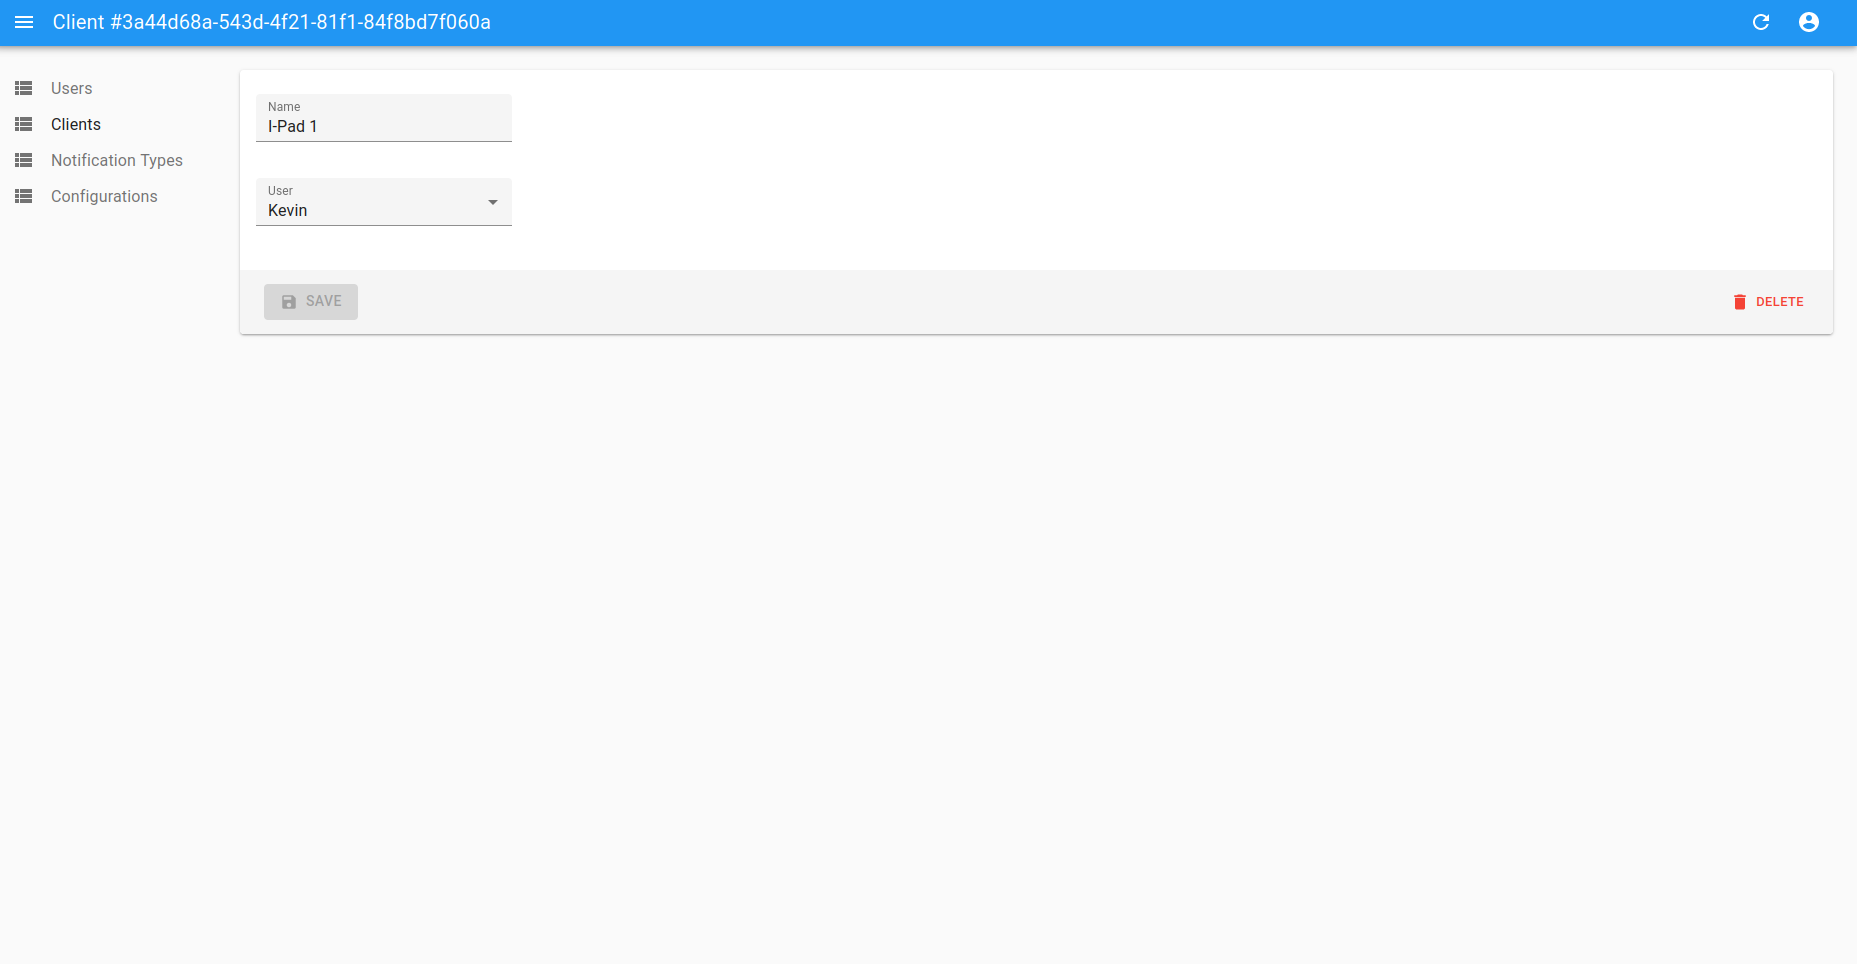
\includegraphics[width=\textwidth]{graphics/screenshots/adminui/configuration}
        \caption{Login}
    \end{minipage}
    \hfill
    \begin{minipage}[b]{0.4\textwidth}
        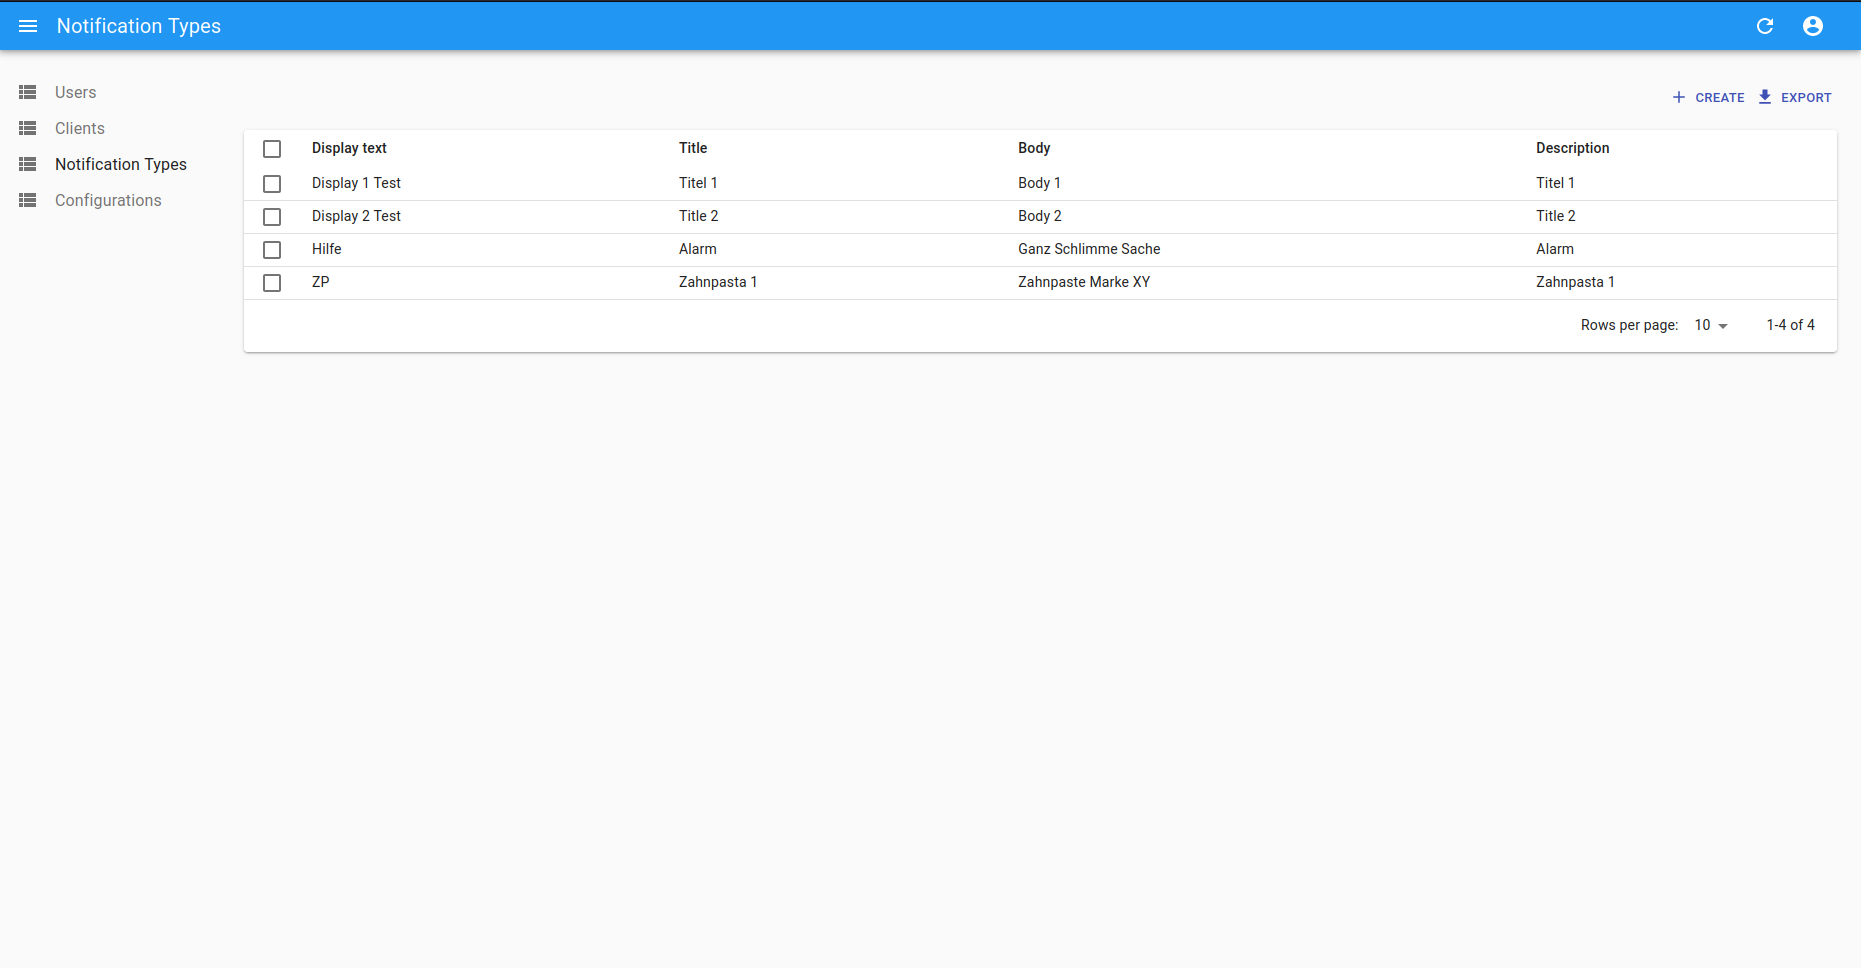
\includegraphics[width=\textwidth]{graphics/screenshots/adminui/notification-type}
        \caption{Configuration Overview}
    \end{minipage}
    \label{fig:AdminUI-Screens2}
\end{figure}




Add some screen shots

\subsection{Tests}

\subsubsection*{Benutzertests}
Wurden mit Daniel Jossen zusannem an der FH gemacht.
Mehr Tests waren wegen Ferienabwesenheiten auf Kundenseite nicht möglich.
Macht nicht so viel sinn mit nur einem Ipad.


\subsubsection*{Benutzertests}
Macht nicht so viel sinn mit nur einem Ipad.

\clearpage
\subsection{Lessons Learned}

\clearpage
\begin{itemize}
    \item Die Gegensprechanlage ist komplett Weggefallen.
    \subitem Grundsätzlich Stünde eine Lib. für IOS in NS zur Verfügung. Der Android Teil ist da noch "TODO"
    \item Die Rückfärbung der Buttons auf Grün ist weggefallen da der Handshake so nicht implmentiert wurde.
\end{itemize}


Hearusforderungen waren:
\begin{itemize}
    \item Dokumentation fehlt komplett in der Planung
    \item IOS Recherche viel aufwändiger als erwartet.
    \item Nativescript aufwändiger zu gebrauchen als erwartet.
    \item AWS aufsetzen ist alles andere als trivial
    \item Keine Erfahrung mit Mobile Development
    \item Stärkerer Roter Faden von Anfang an hätte geholfen
    \item Mehr testing, viel Mehr Testing.
    \item Refactoring kostet Zeit, kanns aber wert sein.
\end{itemize}

Darus mitgenommen haben wir:
\begin{itemize}
    \item Gute Planung macht sich bezahlt. (Roter Faden, Doku mit einplanen, Standortbestimmung)
    \item Gute Konzepte machen sich bezahlt.
    \item Best Practices gibt es aus einem Grund. (Nativ ist besser)
    \item DevOps ist schwer.
\end{itemize}





